%Jennifer Pan, August 2011

\documentclass[10pt,letter]{article}
	% basic article document class
	% use percent signs to make comments to yourself -- they will not show up.

\usepackage{amsmath}
\usepackage{amssymb}
\usepackage{enumitem}
\usepackage{tikz}
	% packages that allow mathematical formatting
\DeclareMathOperator*{\argmax}{arg\,max}
\DeclareMathOperator*{\argmin}{arg\,min}
\usepackage{graphicx}
	% package that allows you to include graphics

\usepackage{setspace}
	% package that allows you to change spacing

\onehalfspacing
	% text become 1.5 spaced

\usepackage{fullpage}
	% package that specifies normal margins


\begin{document}
	% line of code telling latex that your document is beginning


\title{ECON500: Problem Set 1}

\author{Nicholas Wu}

\date{Fall 2020}
	% Note: when you omit this command, the current dateis automatically included

\maketitle
	% tells latex to follow your header (e.g., title, author) commands.


\section*{Problem 2}
\paragraph{(15.B.4)}
\begin{enumerate}[label=(\alph*)]
\item See the diagram. Note that as the price of good 2 increases, the quantity of 2 demanded decreases and the quantity of 1 increases.

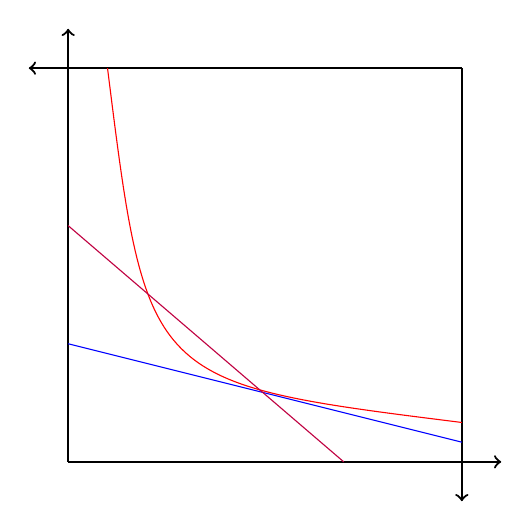
\begin{tikzpicture}
\draw[thick,->] (0,0) -- (5.5,0) ;
\draw[thick,->] (0,0) -- (0,5.5) ;
\draw[thick,->] (5,5) -- (5,-0.5) ;
\draw[thick,->] (5,5) -- (-0.5,5) ;
\draw[red] (0.5,5) .. controls (1,1) .. (5,0.5) ;
\draw[blue] (0,1.5) -- (5,0.25);
\draw[purple] (0,3) -- (3.5,0);
\end{tikzpicture}
\item Suppose, for sake of contradiction, that there are two intersections, at price pairs $(p, 1)$ and $(p', 1)$. WLOG, suppose $p > p'$. Let the allocations at these points be $x$, $x'$. By the gross substitutes property, we must have $x_{11} < x'_{11}$ and $x_{21} < x'_{21}$. But we know that intersections of the offer curves constitute Walrasian equilibria, so we must have by market clearing
\[ x_{11} + x_{21} = \omega_{11} + \omega_{12}  \]
\[ x'_{11} + x'_{21} = \omega_{11} + \omega_{12}  \]
but this is clearly impossible with $x_{11} < x'_{11}$ and $x_{21} < x'_{21}$. Hence, we cannot have multiple intersections of the offer curves outside of the initial endowment if both consumers satisfy gross substitutes.
\item See the diagram. Note that the demand of good 2 does increase at high prices for good 2, but good 1's demand also increases when demand for good 2 increases. Note that this fails gross substitutes.

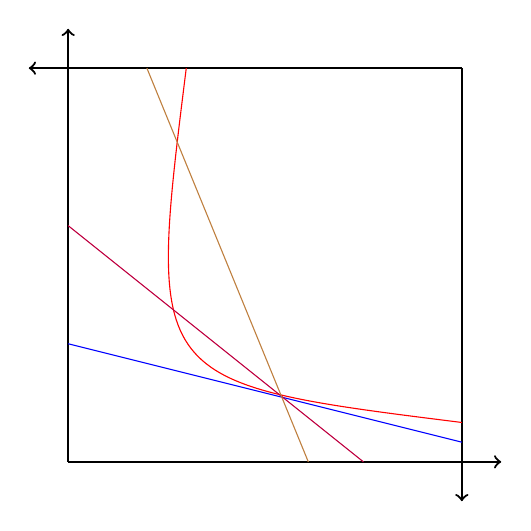
\begin{tikzpicture}
\draw[thick,->] (0,0) -- (5.5,0) ;
\draw[thick,->] (0,0) -- (0,5.5) ;
\draw[thick,->] (5,5) -- (5,-0.5) ;
\draw[thick,->] (5,5) -- (-0.5,5) ;
\draw[red] (1.5,5) .. controls (1,1) .. (5,0.5) ;
\draw[blue] (0,1.5) -- (5,0.25);
\draw[purple] (0,3) -- (3.75,0);
\draw[brown] (1,5) -- (3.05,0);
\end{tikzpicture}
\item See the diagram. Note this demand curve fails normality. Between the purple and brown budget lines, the demand for good 2 increases but the demand for good 1 falls.

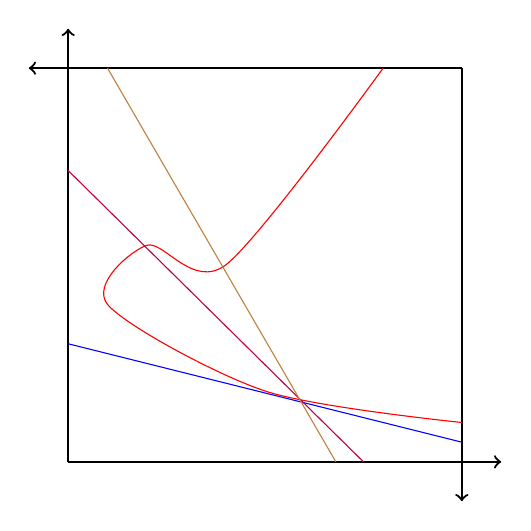
\begin{tikzpicture}
\draw[thick,->] (0,0) -- (5.5,0) ;
\draw[thick,->] (0,0) -- (0,5.5) ;
\draw[thick,->] (5,5) -- (5,-0.5) ;
\draw[thick,->] (5,5) -- (-0.5,5) ;
\draw[red] plot [smooth] coordinates {(4,5) (2,2.5) (1,2.75) (0.5, 2) (2.5, 0.9) (5,0.5)} ;
\draw[blue] (0,1.5) -- (5,0.25);
\draw[purple] (0,3.7) -- (3.75,0);
\draw[brown] (0.5,5) -- (3.4,0);
\end{tikzpicture}
Now, we show that the demand cannot be normal if the offer curve is not normal. Suppose the offer curve is not normal, and consider two price points $(p,1), (p', 1)$, $p' > p$, such that moving on the offer curve from $(p,1)$ to $(p',1)$, the quantity of good 1 demanded increases and the quantity of good 2 demanded decreases. Define $w = p\omega_1 + \omega_2$, $w' = p'\omega_1 + \omega_2 > w$.
\[ x_1(p, w) < x_1(p', w') \]
\[ x_2(p, w) > x_2(p', w') \]
If good 2 is inferior, we are done. Otherwise, since $x_2(p,w) > x_2(p',w')$, it must be the case that real wealth has decreased from $(p,w)$ to $(p',w')$. But since the consumption of good 1 increased as real wealth decreased from $(p,w)$ to $(p',w')$, it must be the case then that good 1 is inferior. Hence at least one of the goods is inferior, and so the demand is not normal.
\item Suppose we have multiple intersections, at prices $(p,1)$ and $(p',1)$, $p' > p$. Let the allocations at these points be $x$, $x'$. By the gross substitutes property, we must have $x_{11} < x'_{11}$ and $x_{12} > x'_{12}$. Further, by normality, we require either $x_{21} < x'_{21}$ or both of $x_{21} > x'_{21}$ and $x_{22} > x'_{22}$.

But we know that intersections of the offer curves constitute Walrasian equilibria, so we must have by market clearing
\[ x_{11} + x_{21} = \omega_{11} + \omega_{21}  \]
\[ x_{12} + x_{22} = \omega_{12} + \omega_{22}  \]
\[ x'_{11} + x'_{21} = \omega_{11} + \omega_{21}  \]
\[ x'_{12} + x'_{22} = \omega_{12} + \omega_{22}  \]
Importantly, we require
\[ x_{11} + x_{21} = x'_{11} + x'_{21} \]
\[ x_{12} + x_{22} = x'_{12} + x'_{22} \]
Since $x_{11} < x'_{11}$, we must have $x_{21} > x'_{21}$. But by normality, this necessitates that $x_{22} > x'_{22}$, and by gross substitutes, $x_{12} > x'_{12}$. But these imply $x_{12} + x_{22} > x'_{12} + x'_{22}$, a contradiction. Hence, we can only have one intersection of the offer curves if one consumer has gross substitutes and the other is normal.

\item See the diagram below. There are many intersection points for these two offer curves.

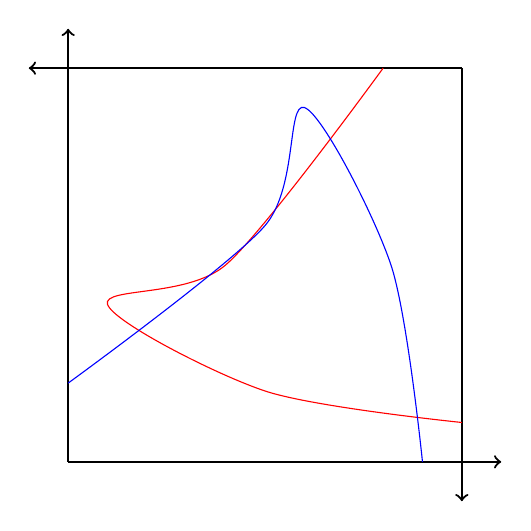
\begin{tikzpicture}
\draw[thick,->] (0,0) -- (5.5,0) ;
\draw[thick,->] (0,0) -- (0,5.5) ;
\draw[thick,->] (5,5) -- (5,-0.5) ;
\draw[thick,->] (5,5) -- (-0.5,5) ;
\draw[red] plot [smooth] coordinates {(4,5) (2,2.5)  (0.5, 2) (2.5, 0.9) (5,0.5)} ;
\draw[blue] plot [smooth] coordinates {(0, 1) (2.5,3) (3,4.5) (4.1,2.5) (4.5, 0)};
\end{tikzpicture}
\end{enumerate}
\paragraph{(15.B.8)} Let the two utility functions be
\[ u_1(x,y) = x + f(y) \]
\[ u_2(x,y) = x + g(y) \]
If preferences are strictly convex, then
\[  x +  f(\lambda y + (1-\lambda)y')  > \lambda (x+f(y)) + (1-\lambda)(x + f(y')) \]
\[ f(\lambda y + (1-\lambda)y')> \lambda f(y) + (1-\lambda) f(y')  \]
Similarly for $g$. So both $f$ and $g$ are strictly concave.

By the second welfare theorem, any Pareto optimal allocation is supported by some prices and endowment choices. Normalize the numeraire price to 1. Let some interior Pareto optimal allocation be supported by the price vector $(1, p)$. By the optimization FOCs, since the allocation is interior, we require
\[ 1 - \lambda = 0 \]
\[ f'(y_1) - \lambda p =0 \]
or
\[ f'(y_1) = p \]
Similarly,
\[ g'(y_2) = p \]
Let the aggregate endowment of $y$ be $\omega_y$. Then at any Pareto optimal allocation, we must have
\[ f'(y_1) = g'(\omega_y - y_1) = p \]
\[ f'(y_1) - g'(\omega_y - y_1) = 0 \]
Define
\[ h(y) = f'(y) - g'(\omega_y - y) \]
Then
\[ h'(y) = f''(y) + g''(\omega_y - y) \]
Due to continuity and strictly convex preferences, both $f''$ and $g''$ are nonzero and have the same sign, and hence $h$ is a strictly monotonic function. Therefore, $h(y) = 0$ for at most one unique value of $y$, and since $y_1$ satisfies $h(y_1) = 0$, we know that since any interior Pareto optimal allocation must satisfy $h(y) = 0$, any interior Pareto optimal allocation always assigns $y_1$ to consumer 1 and $\omega_y - y_1$ to consumer 2.

\section*{Problem 3}
We know from the first half of this course that since preferences are strictly convex, the demand correspondence is a function and hence single-valued. It remains to show that the demand is indeed smooth.
By definition, we have
\[ x_i(p,w) = \argmax_{p\cdot x \le w \cdot } u(x) \]
The FOCs require
\[ u_1(x_i(p,w)) - \lambda p = 0 \]
\[ u_2(x_i(p,w)) - \lambda = 0 \]
\[ (p,1) \cdot x_i(p,w) - w  = 0\]
Stacking the LHS into a vector, we have
\[ v = \begin{bmatrix}
  u_1(x_i(p,w)) - \lambda p \\
  u_2(x_i(p,w)) - \lambda  \\
  (p, 1) \cdot x_i(p,w) - w
\end{bmatrix} \]
The bordered Hessian is
\[ H = \begin{bmatrix} u_{11} & u_{21} & -p \\ u_{21} & u_{22} & -1 \\ -p & -1 & 0 \\ \end{bmatrix}\]
Assuming $|H| \neq 0$, we can then use the implicit function theorem.
\[ \begin{bmatrix}
  \frac{\partial x_1}{\partial p} & \frac{\partial x_1}{\partial w} \\  \frac{\partial x_2}{\partial p} & \frac{\partial x_2}{\partial w}  \\ \frac{\partial \lambda}{\partial p} & \frac{\partial \lambda}{\partial w}  \\
\end{bmatrix} = H^{-1} (D_{p,w} v) \]
Then we note that the expressions for the partial derivatives of $x_1, x_2$ with respect to $p, w$ are a smooth linear transformation of smooth functions, and hence are smooth. Therefore, since first derivative matrix of $x_1$, $x_2$ is smooth, we have that $x_1, x_2$ are smooth.

To show $x_i$ is a diffeomorphism, it suffices to argue the preimage map $x_i^{-1}$ is a well-defined function and smooth. Suppose that $x^*$ is some consumption bundle for player $i$, where $x^*$ is part of a feasible allocation (inside the Edgeworth box). For well-definedness, it suffices to show that there exists a unique price $p$ and wealth $w$ such that $x_i(p,w) = x^*$. The utility maximization problem is
\[ x_i(p,w) = \argmax_{p\cdot x \le w \cdot } u(x) \]
Let
\[ p = \frac{\frac{\partial u}{\partial x_1} \Bigr|_{ x^*}}{\frac{\partial u}{\partial x_2} \Bigr|_{x^*}} \]
and
\[ w = p x^*_1 + x^*_2  \]
We note that by our assumptions on the utility function (i.e. differentiable and increasing), our expression for $p$ is always positive and well defined, since the denominator is never zero.

Then we note first order conditions for utility maximization are: (assuming (i) - (iii) and strictly convex preferences)
\[ \frac{\partial u}{\partial x_1} \Bigr|_{x^*} = \lambda p \]
\[ \frac{\partial u}{\partial x_2} \Bigr|_{x^*} = \lambda  \]
\[ p \cdot x^* = w  \]
Hence, $p$ uniquely solves these at $x^*$, since $\lambda$ is fully determined from equation 2, so $p$ is fully determined, and hence $w$ is also fully determined. So $x^*$ is feasible and binding under the budget constraint at $(p,w)$. Hence we have that
$x_i(p,w) = x^*$, and so $x_i$ is invertible.

Further, we can examine our expression for $p$:
\[ p(x^*) = \frac{\frac{\partial u}{\partial x_1} \Bigr|_{x^*}}{\frac{\partial u}{\partial x_2} \Bigr|_{x^*}} \]
Since $u$ is assumed to be smooth, we know that the partial derivatives of $u$ with respect to $x_1$ and $x_2$ are also smooth. Now, we note the transformation $f(x,y) = x/y$ is smooth for $x,y > 0$, and $u_1, u_2 > 0$, we know that since a composition of smooth functions is smooth, we have that $p(x^*)$ is smooth. Similarly, since $w(x^*) = p(x^*) x^*_1 + x^*_2$ is also a composition of a smooth function and $p$ is smooth, $w$ is also smooth. Therefore, we have the preimage of demand under fixation of the numeraire price of good 2 is well-defined and smooth, so $x_i$ is a diffeomorphism between the 2-manifolds of the consumption space and the price/wealth $(p,w)$ space (where $p$ is the price of good 2).

\section*{Problem 4}

The offer curve is $\mathcal{O}_i = \{ x_i(p', p' \cdot \omega) \ : \ p' = (p, 1) > 0 \} $ where we have normalized the price of good 2 to 1 as the numeraire.
Now, since $x_i$ is a diffeomorphism (we showed this in the previous problem) we have that since the offer curve is the image of the line $p \omega_1 + \omega_2 = w$ under the mapping $x_i$. Since $x_i$ is smooth, and the line $p \omega_1 + \omega_2 = w$ is smooth in the $(p,w)$ space, we have that the offer curve is also smooth. Further, we note that using the inverse we computed in the previous problem,
\[ x_i \left( \frac{u_1(\omega)}{u_2(\omega)}, \frac{u_1(\omega)}{u_2(\omega)}\omega_1  + \omega_2 \right) = \omega \]
And we note that
\[ \left( \frac{u_1(\omega)}{u_2(\omega)}, \frac{u_1(\omega)}{u_2(\omega)}\omega_1  + \omega_2 \right) \]
lies on the offer curve preimage $p \omega_1 + \omega_2 = w$. Hence the offer curve passes through the endowment.

The indifference curve at $\omega$ is given by the equation:
\[ u_i(x_1, x_2) = u_i(\omega) \]
It follows that since $u_i$ is smooth, and $u_i(\omega)$ is a constant, the indifference curve is smooth, since the normal vector to $I(\omega)$ is (assuming smoothness of $u$)
\[ (u_1(x_1, x_2), u_2(x_1, x_2)) \]
which varies continuously in $x_1, x_2$.

Finally, we know that at each point on the offer curve, since $x_i$ maximizes utility and $\omega$ is in the budget set, for any $x \neq \omega$, $x \in \mathcal{O}_i$, $u(x) \ge u(\omega)$. Now, suppose $\mathcal{O}$ is not tangent to $I(\omega)$ at $\omega$. This implies that $\mathcal{O}$ must cross $I(\omega)$ at $\omega$, which means since $u$ is increasing, for any neighborhood of $\omega$, there exist points $x', x''$ such that $u(x') > u(\omega)$ and $u(x'') < u(\omega)$. But $x', x''$ cannot both lie on the offer curve, a contradiction. Hence we must have that $\mathcal{O}$ is tangent to $I(\omega)$ at $\omega$.

Now, we already showed that the offer curve is smooth, and is the image of the line $p \omega_1 + \omega_2 = w$ under $x_i$. Fix some bundle $x^* \in \mathcal{O}_i$, and let $p^*$ be the price that yields the offer $x^*$. We know $x^* = x_i(p^*, p^*\cdot \omega)$, so the normal vector is given by
\[ \lambda(x^*) = \nabla x_i(p^*, p^* \cdot \omega) \] From problem 3, we argued by the implicit function theorem that $x_i$ was smooth in $p, w$, and hence is smooth under the parametrization $p^*, p^* \cdot \omega$. Therefore,
$ \lambda(x^*) $ is continuously differentiable.

\end{document}
	% line of code telling latex that your document is ending. If you leave this out, you'll get an error
